\documentclass[11pt,a4paper]{article}
\usepackage[margin=2.3cm]{geometry}
\usepackage{amsmath,amssymb,amsthm}
\usepackage{booktabs}
\usepackage{graphicx}
\usepackage{microtype}
\usepackage[font=small,labelfont=bf]{caption}
\usepackage[colorlinks=true,linkcolor=black,citecolor=black,urlcolor=blue!50!black]{hyperref}
\usepackage{xcolor}
\usepackage[authoryear,round]{natbib}
% generated by code/make_numbers.py -- do not edit
\newcommand{\ZeroFracFullAll}{66.9}
\newcommand{\ZeroPairsTotal}{1,048,576}
\newcommand{\ZeroPairsFull}{701,944}
\newcommand{\ZeroMeanClass}{1.94}
\newcommand{\ZeroMaxClass}{128}
\newcommand{\ZeroMaxTau}{240}
\newcommand{\ZeroMedianTau}{12}
\newcommand{\ZeroMeanTau}{14.7}
\newcommand{\ZeroMaxTauRule}{45}
\newcommand{\ZeroClassHist}{$|C_\infty|=1$: 66.9\%, $|C_\infty|=2$: 21.6\%, $|C_\infty|=4$: 6.5\%, $|C_\infty|=8$: 3.4\%, $|C_\infty|=16$: 1.4\%, $|C_\infty|=32$: 0.1\%, larger: 0.07\%}
\newcommand{\ZeroBestClassFrac}{99.8}
\newcommand{\ZeroBestClassRule}{25 and 60}
\newcommand{\ZeroWorstClassFrac}{19.0}
\newcommand{\ZeroWorstClassRules}{170, 204}
\newcommand{\NumClassesBproved}{42}
\newcommand{\NumClassesUndet}{46}
\newcommand{\NumRulesBproved}{138}
\newcommand{\NumRulesUndet}{118}
\newcommand{\NumClassesAllCyclesFull}{0}
\newcommand{\StatEntries}{1496}
\newcommand{\StatUnresolved}{13}
\newcommand{\StatUnresolvedRules}{7, 19, 23, 232}
\newcommand{\StatUnresolvedEpsMax}{0.010}
\newcommand{\StatMaxResidual}{4.7e-13}
\newcommand{\StatMaxCheckDevResolved}{5.2e-08}
\newcommand{\EpsGrid}{0.001, 0.002, 0.005, 0.01, 0.02, 0.03, 0.05, 0.075, 0.1, 0.125, 0.15, 0.2, 0.25, 0.3, 0.35, 0.4, 0.45, 0.5}
\newcommand{\EpsGridN}{18}
\newcommand{\SymmetryWorstDev}{5.9e-11}
\newcommand{\SymmetryPairs}{12,972}
\newcommand{\SymmetryChecked}{yes}
\newcommand{\NumInterior}{61}
\newcommand{\NumBoundaryMax}{26}
\newcommand{\NumInteriorB}{42}
\newcommand{\NumInteriorU}{19}
\newcommand{\NumBoundaryB}{0}
\newcommand{\NumBoundaryU}{26}
\newcommand{\EpsStarMin}{0.010}
\newcommand{\EpsStarMax}{0.293}
\newcommand{\EpsStarMedian}{0.132}
\newcommand{\EpsStarMinRule}{106}
\newcommand{\EpsStarMaxRule}{128}
\newcommand{\RhoStarMin}{0.1101}
\newcommand{\RhoStarMax}{6.189}
\newcommand{\RhoStarMinRule}{0}
\newcommand{\RhoStarMaxRule}{106}
\newcommand{\SpearmanEpsStarFrac}{$-0.44$}
\newcommand{\SpearmanEpsStarClass}{$+0.64$}
\newcommand{\SpearmanPFrac}{4\cdot10^{-4}}
\newcommand{\SpearmanPClass}{4\cdot10^{-8}}
\newcommand{\ArgminSevenCount}{41}
\newcommand{\ArgminZeroCount}{5}
\newcommand{\NumSignChangesGtOne}{2}
\newcommand{\SignChangesGtOneRules}{41, 108}
\newcommand{\NumRisingB}{0}
\newcommand{\NumRisingU}{27}
\newcommand{\NumFallingU}{19}
\newcommand{\NumRisingUInterior}{1}
\newcommand{\RisingUInteriorRules}{41}
\newcommand{\RisingTrendMin}{0.850}
\newcommand{\RisingTrendMax}{0.986}
\newcommand{\TrendLateRules}{7 (0.02/0.03), 19 (0.01/0.02), 23 (0.01/0.02), 232 (0.01/0.02)}
\newcommand{\TrendSecondEpsMax}{0.03}
\newcommand{\FallingUTrendMin}{1.430}
\newcommand{\FallingBTrendMin}{1.662}
\newcommand{\UniformMarginalRules}{15, 51, 60, 90, 105, 150, 170, 204}
\newcommand{\NumUniformMarginal}{8}
\newcommand{\UniformMarginalMaxDev}{4.2e-12}
\newcommand{\BijectiveRules}{15, 51, 170, 204}
\newcommand{\NumBijective}{4}
\newcommand{\AffineNonBijRules}{60, 90, 105, 150}
\newcommand{\NumAffineNonBij}{4}
\newcommand{\AffineKernelDims}{1, 2, 2, 2}
\newcommand{\AffineBadCharacters}{0}
\newcommand{\AffineMinPi}{1.3e-04}
\newcommand{\UniformMarginalRhoSmall}{10.339}
\newcommand{\LambdaSmall}{6.893}
\newcommand{\NumRefineUnresolved}{0}
\newcommand{\BoundaryMaxRules}{5, 9, 15, 22, 25, 27, 29, 30, 37, 45, 51, 54, 60, 62, 73, 74, 90, 105, 108, 110, 122, 150, 154, 170, 184, 204}
\newcommand{\RuleZeroNuSevenCheck}{4.1e-14}
\newcommand{\RuleZeroEpsStar}{0.292}
\newcommand{\RuleZeroRhoStar}{0.1101}
\newcommand{\RuleZeroStepsPerNat}{9}
\newcommand{\EpsStarRuleThirty}{--}
\newcommand{\RhoStarRuleThirty}{--}
\newcommand{\TypeRuleThirty}{U}
\newcommand{\RhoSmallRuleThirty}{8.517}
\newcommand{\RhoMidRuleThirty}{2.637}
\newcommand{\EpsStarRuleOneTen}{--}
\newcommand{\RhoStarRuleOneTen}{--}
\newcommand{\TypeRuleOneTen}{U}
\newcommand{\RhoSmallRuleOneTen}{4.479}
\newcommand{\RhoMidRuleOneTen}{1.484}
\newcommand{\EpsStarRuleTwoOhFour}{--}
\newcommand{\RhoStarRuleTwoOhFour}{--}
\newcommand{\TypeRuleTwoOhFour}{U}
\newcommand{\RhoSmallRuleTwoOhFour}{10.339}
\newcommand{\RhoMidRuleTwoOhFour}{2.637}
\newcommand{\EpsStarRuleTwoThreeTwo}{0.119}
\newcommand{\RhoStarRuleTwoThreeTwo}{1.040}
\newcommand{\TypeRuleTwoThreeTwo}{U}
\newcommand{\RhoSmallRuleTwoThreeTwo}{0.041}
\newcommand{\RhoMidRuleTwoThreeTwo}{1.025}
\newcommand{\EpsStarRuleOneTwoEight}{0.293}
\newcommand{\RhoStarRuleOneTwoEight}{0.130}
\newcommand{\TypeRuleOneTwoEight}{B}
\newcommand{\RhoSmallRuleOneTwoEight}{0.000}
\newcommand{\RhoMidRuleOneTwoEight}{0.022}
\newcommand{\EpsStarRuleEighteen}{0.147}
\newcommand{\RhoStarRuleEighteen}{0.465}
\newcommand{\TypeRuleEighteen}{B}
\newcommand{\RhoSmallRuleEighteen}{0.013}
\newcommand{\RhoMidRuleEighteen}{0.433}
\newcommand{\EpsStarRuleNinety}{--}
\newcommand{\RhoStarRuleNinety}{--}
\newcommand{\TypeRuleNinety}{U}
\newcommand{\RhoSmallRuleNinety}{10.339}
\newcommand{\RhoMidRuleNinety}{2.637}
\newcommand{\UndetBoundaryRatioMin}{0.850}
\newcommand{\UndetBoundaryRatioMax}{0.954}
\newcommand{\GridMaxRhoOverall}{10.339}
\newcommand{\GridMaxRhoRule}{90}
\newcommand{\GridMaxRhoEps}{0.001}
\newcommand{\FHallaA}{67.9}
\newcommand{\FHgtaA}{12.0}
\newcommand{\FHallaB}{75.5}
\newcommand{\FHgtaB}{41.4}
\newcommand{\FHallaC}{83.6}
\newcommand{\FHgtaC}{63.1}
\newcommand{\FHallaD}{87.4}
\newcommand{\FHgtaD}{73.1}
\newcommand{\FHallbA}{68.3}
\newcommand{\FHgtbA}{28.5}
\newcommand{\FHallbB}{76.7}
\newcommand{\FHgtbB}{50.7}
\newcommand{\FHallbC}{85.3}
\newcommand{\FHgtbC}{71.9}
\newcommand{\FHallbD}{89.2}
\newcommand{\FHgtbD}{80.5}
\newcommand{\FHallcA}{77.7}
\newcommand{\FHgtcA}{63.2}
\newcommand{\FHallcB}{85.4}
\newcommand{\FHgtcB}{77.7}
\newcommand{\FHallcC}{90.1}
\newcommand{\FHgtcC}{84.2}
\newcommand{\FHallcD}{93.2}
\newcommand{\FHgtcD}{89.4}
\newcommand{\FHalldA}{79.6}
\newcommand{\FHgtdA}{69.7}
\newcommand{\FHalldB}{88.0}
\newcommand{\FHgtdB}{82.4}
\newcommand{\FHalldC}{93.1}
\newcommand{\FHgtdC}{90.3}
\newcommand{\FHalldD}{95.6}
\newcommand{\FHgtdD}{93.9}
\newcommand{\FHalleA}{73.1}
\newcommand{\FHgteA}{63.2}
\newcommand{\FHalleB}{89.9}
\newcommand{\FHgteB}{86.8}
\newcommand{\FHalleC}{96.7}
\newcommand{\FHgteC}{95.7}
\newcommand{\FHalleD}{100.0}
\newcommand{\FHgteD}{100.0}
\newcommand{\FHlnThreshold}{4.61}
\newcommand{\FHpooledGtaC}{51.8}
\newcommand{\FHpooledAllaC}{83.6}
\newcommand{\FHpooledGtbC}{61.4}
\newcommand{\FHpooledAllbC}{85.3}
\newcommand{\FHpooledGtcC}{77.3}
\newcommand{\FHpooledAllcC}{90.1}
\newcommand{\FHpooledGtdC}{85.6}
\newcommand{\FHpooledAlldC}{93.1}
\newcommand{\FHpooledGteC}{93.2}
\newcommand{\FHpooledAlleC}{96.7}
\newcommand{\FHnonIdStatesPerClassMin}{10}
\newcommand{\FHnonIdStatesPerClassMax}{3316}
\newcommand{\FHbestEpsHist}{$\varepsilon=0.01$: 2, $\varepsilon=0.02$: 12, $\varepsilon=0.05$: 10, $\varepsilon=0.1$: 32, $\varepsilon=0.2$: 32}
\newcommand{\FHbestEpsMedian}{0.1}
\newcommand{\RiiMajSilent}{32.6}
\newcommand{\RiiMajDetectMean}{0.07}
\newcommand{\RiiMajDetectMax}{1}
\newcommand{\RiiMajSilentClass}{5.76}
\newcommand{\RiiMajGstarSmall}{232}
\newcommand{\RiiMajGstarAll}{yes}
\newcommand{\RiiMajRatioMid}{16.0}
\newcommand{\RiiMajRatioSmall}{166.0}
\newcommand{\RiiMajRatioLarge}{0.58}
\newcommand{\RiiMajMisfitMax}{2.220}
\newcommand{\RiiMajMarginMax}{0.750}
\newcommand{\RiiMajCrossEps}{0.125}
\newcommand{\RiiParSilent}{1.6}
\newcommand{\RiiParDetectMean}{0.04}
\newcommand{\RiiParDetectMax}{1}
\newcommand{\RiiParSilentClass}{13.69}
\newcommand{\RiiParGstarSmall}{237}
\newcommand{\RiiParGstarAll}{no}
\newcommand{\RiiParRatioMid}{0.0}
\newcommand{\RiiParRatioSmall}{0.0}
\newcommand{\RiiParRatioLarge}{0.00}
\newcommand{\RiiParMisfitMax}{6.000}
\newcommand{\RiiParMarginMax}{0.000}
\newcommand{\RiiParCrossEps}{0.001}
\newcommand{\RiiDefSilent}{7.1}
\newcommand{\RiiDefDetectMean}{4.18}
\newcommand{\RiiDefDetectMax}{16}
\newcommand{\RiiDefSilentClass}{2.46}
\newcommand{\RiiDefGstarSmall}{110}
\newcommand{\RiiDefGstarAll}{yes}
\newcommand{\RiiDefRatioMid}{2.7}
\newcommand{\RiiDefRatioSmall}{4.3}
\newcommand{\RiiDefRatioLarge}{1.48}
\newcommand{\RiiDefMisfitMax}{0.379}
\newcommand{\RiiDefMarginMax}{0.708}
\newcommand{\RiiDefCrossEps}{--}
\newcommand{\ManifestFiles}{10}


\newtheorem{lemma}{Lemma}
\newtheorem{proposition}{Proposition}
\theoremstyle{remark}
\newtheorem{remark}{Remark}
\newcommand{\eps}{\varepsilon}
\newcommand{\R}{\mathcal{R}}
\newcommand{\E}{\mathbb{E}}
\DeclareMathOperator{\KL}{KL}

\title{Rule identifiability in elementary cellular automata\\under dynamical noise}
\author{Frank Peterlein\thanks{Independent researcher, Berlin. ORCID \href{https://orcid.org/0009-0002-1886-1303}{0009-0002-1886-1303}. Contact: \texttt{frnkptrln} on GitHub. See the statement on the use of AI at the end of the note.}}
\date{Version 0.1 --- 15 October 2026}

\begin{document}
\maketitle

\begin{abstract}
\noindent
How well can the rule of an elementary cellular automaton be read off a trajectory when the dynamics itself is noisy? On a ring of $n=12$ cells the noisy automaton is a Markov chain on $4096$ states, so every quantity in this note is computed exactly: no sampling, no seeds. Without noise, identifiability is combinatorial. A trajectory fixes the rule on the neighbourhoods it visits and on nothing else; the visited set stops growing once the orbit closes; over all $256$ rules and $4096$ initial states, \ZeroFracFullAll\% of the pairs determine the rule and the remaining pairs never do. With dynamical noise every trajectory law has full support and identifiability becomes a rate: the evidence against the hardest alternative grows linearly in time, at $\rho(f;\eps)=\lambda(\eps)\,\min_c\nu_c(f;\eps)$ nats per step, the product of a pure noise factor and the stationary frequency of the rarest neighbourhood. For \NumClassesBproved{} of the $88$ rule classes some neighbourhood occurs on no cycle of the deterministic map, so $\rho$ vanishes at both ends of $[0,\tfrac12]$ and the best noise level is interior; \NumFallingU{} further classes behave the same way, and \NumRisingU{} keep rising as $\eps\to0$. For the \NumInterior{} falling classes we locate the best noise level, $\eps^*\in[\EpsStarMin,\EpsStarMax]$. Noise therefore does not help uniformly: it helps exactly those rules whose noise-selected attractors exercise only part of the rule table. At finite horizon the same mechanism rescues initial states that are permanently non-identifiable without noise. A boundary check with generators outside the family shows the flip side: the observer converges confidently to the nearest rule in its family, while the misfit becomes visible at a lower rate.
\end{abstract}

\section{Definitions}

\paragraph{1.1 Setting.}
Fix $n\ge3$ (computed case: $n=12$). States are $x\in S=\{0,1\}^n$ on a ring. An elementary rule is a map $f:\{0,1\}^3\to\{0,1\}$; $\R$ is the set of all $256$ \citep{Wolfram1983}. The global map is $(F_f x)_i=f(x_{i-1},x_i,x_{i+1})$, indices mod $n$. The neighbourhood set of a state is $N(x)=\{(x_{i-1},x_i,x_{i+1}):i\}\subseteq\{0,1\}^3$; we write $c\in\{0,\dots,7\}$ for the code $4x_{i-1}+2x_i+x_{i+1}$ and $n_c(x)$ for the number of positions of $x$ with code $c$, so that $\sum_c n_c(x)=n$.

\paragraph{1.2 Dynamics.}
For $\eps\in[0,\tfrac12]$: $X_0=x_0$, $X_{t+1}=F_f(X_t)\oplus Z_t$, with $Z_t$ i.i.d.\ vectors of independent Bernoulli($\eps$) bits. The transition kernel is
\[
P_{f,\eps}(y\mid x)=\eps^{H(y,F_f x)}(1-\eps)^{\,n-H(y,F_f x)},
\]
$H$ the Hamming distance. Noise acts on the state and propagates; it is not a noisy readout of a deterministic orbit (Remark~\ref{rem:dyn}).

\paragraph{1.3 Observation and hypotheses.}
The observer sees the full trajectory $x_{0:T}$ and knows $\R$, $\eps$ and $x_0$. The unknown is $f$. The object of study is the family of trace laws $P^T_{f,\eps}(\cdot\mid x_0)$ on $S^T$, $f\in\R$.

\paragraph{1.4 $\eps=0$: combinatorial identifiability.}
Let $x_t$ be the orbit of $f$ from $x_0$ and $N_T(f,x_0)=\bigcup_{t<T}N(x_t)$. The consistent set is
\[
C_T(f,x_0)=\{g\in\R:F_g(x_t)=x_{t+1}\ \forall t<T\}=\{g:g=f\text{ on }N_T(f,x_0)\},\qquad |C_T|=2^{\,8-|N_T|}.
\]
For fixed $(x_0,T)$ this is an equivalence relation on $\R$. Since the orbit is eventually periodic, $N_T$ is non-decreasing in $T$ and constant for $T\ge\tau(f,x_0)$ (transient plus period). The class therefore never shrinks below $2^{8-|N_\infty|}$: after $\tau$, watching longer buys nothing.

\paragraph{1.5 $\eps>0$: quantitative identifiability.}
For $0<\eps<\tfrac12$ every trace law has full support on $S^T$, so $C_T=\R$ and identifiability must be graded. Define the \emph{evidence} against $g$ when $f$ is true,
\[
E_T(f\|g;x_0,\eps)=\KL\!\big(P^T_{f,\eps}(\cdot\mid x_0)\,\big\|\,P^T_{g,\eps}(\cdot\mid x_0)\big)=\E_f\!\left[\log\frac{P_f(X_{1:T}\mid x_0)}{P_g(X_{1:T}\mid x_0)}\right].
\]

\begin{lemma}[decomposition]\label{lem:decomp}
With $d_{fg}(x)=H(F_fx,F_gx)$ and $\lambda(\eps)=(1-2\eps)\log\frac{1-\eps}{\eps}$,
\[
E_T(f\|g;x_0,\eps)=\lambda(\eps)\sum_{t=0}^{T-1}\E_f[\,d_{fg}(X_t)\,].
\]
\end{lemma}
\begin{proof}
Chain rule of relative entropy along the Markov chain \citep[Thm.~2.5.3]{CoverThomas}: $E_T=\sum_t\E_f[\KL(P_f(\cdot\mid X_t)\|P_g(\cdot\mid X_t))]$. Given $x$, $\log\frac{P_f(y\mid x)}{P_g(y\mid x)}=\big(H(y,F_gx)-H(y,F_fx)\big)\log\frac{1-\eps}{\eps}$; bits where $F_fx$ and $F_gx$ agree contribute $0$, each of the $d_{fg}(x)$ bits where they differ contributes $+1$ with probability $1-\eps$ and $-1$ with probability $\eps$, i.e.\ $1-2\eps$ in expectation.
\end{proof}

\emph{Margin and rate.} $m_T(f;x_0,\eps)=\min_{g\ne f}E_T(f\|g;x_0,\eps)$ is the evidence against the hardest alternative. For $\eps>0$ the kernel is strictly positive, hence the chain is ergodic with a unique stationary law $\pi_{f,\eps}$ of full support \citep{Norris}, and $E_T/T\to\lambda(\eps)\E_{\pi_{f,\eps}}[d_{fg}]$. The \emph{identifiability rate} of a rule is
\[
\rho(f;\eps)=\min_{g\ne f}\lambda(\eps)\,\E_{\pi_{f,\eps}}[\,d_{fg}\,],
\]
independent of $x_0$. $\rho$ is constant on the $88$ classes of rules under reflection and complementation \citep{LiPackard1990}, since the chain is equivariant under both.

\begin{lemma}[the hardest alternative is a one-bit neighbour]\label{lem:onebit}
Let $\nu_c(f;\eps)=\E_{\pi_{f,\eps}}[n_c]$ be the expected number of positions with code $c$ under the stationary law. Then $\E_\pi[d_{fg}]=\sum_c\nu_c\,\mathbf 1[f(c)\ne g(c)]$, and
\[
\rho(f;\eps)=\lambda(\eps)\,\min_{c}\nu_c(f;\eps),
\]
the minimum being attained by the rule that differs from $f$ only on the rarest code. The same holds termwise at finite horizon: $m_T(f;x_0,\eps)=\lambda(\eps)\min_c\sum_{t<T}\E_f[n_c(X_t)]$.
\end{lemma}
\begin{proof}
$d_{fg}(x)$ counts the positions whose code lies in the set where $f$ and $g$ differ, so $d_{fg}(x)=\sum_c n_c(x)\mathbf 1[f(c)\ne g(c)]$; take expectations. The sum over a non-empty set of non-negative terms is at least its smallest term, with equality for a singleton.
\end{proof}

\begin{lemma}[ends of the curve]\label{lem:ends}
$\rho(f;\tfrac12)=0$ because $\lambda(\tfrac12)=0$. As $\eps\to0$, every limit point of $\pi_{f,\eps}$ is a stationary law of the deterministic map, i.e.\ a mixture of the uniform laws on the cycles of $F_f$. If some code $c$ occurs in no state of any cycle of $F_f$, then $\nu_c(f;\eps)=O(\eps)$ while $\lambda(\eps)=O(\log\frac1\eps)$, hence $\rho(f;\eps)\to0$: the curve vanishes at both ends and attains its maximum in the interior of $(0,\tfrac12)$; we write $\eps^*(f)$ for a maximiser (uniqueness is not asserted). If instead every code occurs on some cycle that carries positive weight in the small-noise limit, $\min_c\nu_c$ stays bounded away from $0$ and $\rho(f;\eps)\to\infty$.
\end{lemma}
\begin{proof}
For the first statement: $\eps\mapsto P_{f,\eps}$ is continuous and the simplex is compact, so every limit point $\pi_0$ of $\pi_{f,\eps}$ satisfies $\pi_0=\pi_0P_{f,0}$, and the stationary laws of a map are exactly the mixtures of uniform laws on its cycles. For the $O(\eps)$ bound let $A$ be the set of cycle states and $B=S\setminus A$, and let $L$ be the longest transient. From any state the chain follows the deterministic map for one step with probability $(1-\eps)^n\ge1-n\eps$, so a sojourn in $B$ ends within $L$ steps unless a noise event occurs during those steps; the expected sojourn length is therefore at most $L/(1-n\eps)^L$. A sojourn in $B$ can only start by a noise event from $A$, which has probability at most $n\eps$ per step. By the renewal structure of the stationary chain, $\pi_{f,\eps}(B)\le n\eps\,L/(1-n\eps)^L=O(\eps)$. A code that occurs on no cycle occurs only in $B$, so $\nu_c\le n\,\pi_{f,\eps}(B)=O(\eps)$. The last statement follows from $\nu_c\to\sum_{\text{cycles }C}w_C\,\overline{n_c}(C)$ with the limiting weights $w_C$ \citep{FreidlinWentzell}.
\end{proof}

Which cycles carry weight in the small-noise limit is a question about the large-deviation costs between basins \citep{FreidlinWentzell}; this note does not compute those weights. It uses the checkable sufficient condition of Lemma~\ref{lem:ends} (a code absent from every cycle), and reports the numerical trend of $\rho$ at the smallest resolved noise levels for the remaining classes.

\begin{remark}[why the noise must be dynamical]\label{rem:dyn}
If instead a readout channel $K$ corrupts the deterministic orbit, the trace law is $K\circ P_{f,0}$, and by the data-processing inequality the evidence $E_T$ can only decrease; in particular rules that the orbit does not separate ($g\in C_T(f,x_0)$, equal trace laws) remain inseparable under every readout channel. ``Noise increases identifiability'' is a statement about noise in the dynamics only.
\end{remark}

\begin{remark}[what the evidence licenses]\label{rem:bh}
For any decision rule, i.e.\ any event $A$, $P_f(A^c)+P_g(A)\ge\tfrac12\exp(-E_T(f\|g))$ \citep{BretagnolleHuber1979,Tsybakov2009}. A small margin therefore bounds from below the confusion of $f$ with its hardest alternative under \emph{every} procedure; this is the direction that establishes non-identifiability. Upper bounds on the error of the maximum-likelihood decoder can be added via Chernoff exponents; this note reports $E$, $m$ and $\rho$ exactly and does not report decoder error rates.
\end{remark}

\paragraph{1.6 Declared boundaries.}
The true rule lies in $\R$; $\eps$ is known to the observer; observation is complete; $n=12$ on a ring. Each is a boundary of the claim, not an experiment of this note; Section~\ref{sec:boundary} probes the first of them with a check, not with a theorem.

\section{Computation}\label{sec:comp}

Every number in this note is a function of the $4096$-state chain and is computed as such.

\emph{Stationary laws.} For each rule and each $\eps$ on the grid $\eps\in\{$\EpsGrid$\}$ (\EpsGridN{} values; at $\eps=\tfrac12$ the stationary law is uniform and $\rho=0$ analytically), $\pi_{f,\eps}$ is obtained by solving the linear system $\pi(I-P_{f,\eps})=0$, $\sum\pi=1$, with the dense $4096\times4096$ transition matrix. The solution is then verified by power iteration from three different initial laws (uniform, and the point masses at the all-zero and the all-one state): an entry is \emph{resolved} when all three converge to the dense solution to within $10^{-6}$ in every $\nu_c$; otherwise the chain is metastable at that $\eps$ (it mixes too slowly for the stationary law to be resolved numerically), and the entry is excluded from everything that follows. Over the $88$ class representatives, \StatUnresolved{} of \StatEntries{} entries are unresolved (rules \StatUnresolvedRules, all at $\eps\le\StatUnresolvedEpsMax$). The largest residual $\|\pi-\pi P\|_1$ among the dense solutions is \StatMaxResidual; the largest deviation between the dense solution and any power iteration among resolved entries is \StatMaxCheckDevResolved.

\emph{Best noise level.} For every class whose grid maximum of $\rho$ is interior, $\eps^*$ is located by golden-section search between the neighbouring grid points to a width of $5\cdot10^{-4}$, each evaluation being a dense solve, and the solution at $\eps^*$ is verified as above.

\emph{Symmetry check.} The chain is equivariant under reflection and complementation, so $\nu_c$ for the image of a rule under either symmetry is a permutation of $\nu_c$ for the rule itself (for a self-symmetric rule a constraint on its own $\nu_c$). All $256$ rules were computed independently; over the \SymmetryPairs{} pairs of a rule, a symmetry and a grid point at which the class representative is resolved, the largest deviation from the predicted permutation is \SymmetryWorstDev.

\emph{Zero noise.} For each of the $256\times4096$ pairs $(f,x_0)$ the orbit is followed until it closes; this yields $\tau(f,x_0)$, $N_\infty(f,x_0)$ and $|C_\infty|$ exactly.

\emph{Finite horizon.} $\sum_{t<T}\E_f[n_c(X_t)\mid x_0]$ for all $4096$ initial states at once is computed backwards, $G_t=P_{f,\eps}G_{t-1}$ with $G_0$ the $4096\times8$ matrix of counts, using the tensor-product structure of the noise kernel; this is exact and costs $O(8n\,2^n)$ per step.

\emph{Analytic check.} For rule $0$ the chain is a sequence of independent Bernoulli($\eps$) vectors, so $\nu_7=n\eps^3$ exactly; the computed values deviate from $12\eps^3$ by at most \RuleZeroNuSevenCheck.

The whole computation runs in about two hours on two CPU cores. Code, data and a SHA-256 manifest of the \ManifestFiles{} data files accompany the note.

\section{Results}\label{sec:results}

\subsection{Zero noise}

\begin{figure}[t]
\centering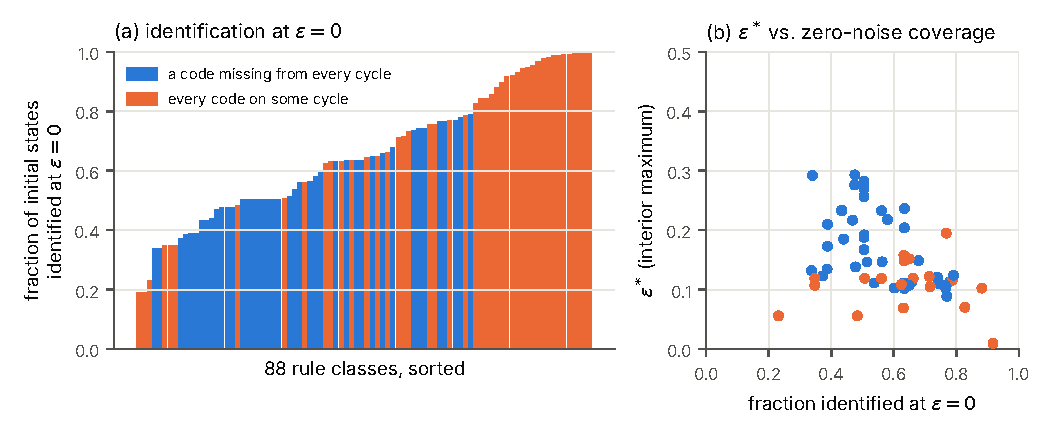
\includegraphics[width=\textwidth]{figures/fig_zero_noise.pdf}
\caption{(a) Fraction of the $4096$ initial states from which the orbit determines the rule ($|C_\infty|=1$), for each of the $88$ rule classes, sorted. Blue: some neighbourhood code occurs on no cycle of the deterministic map (\NumClassesBproved{} classes); orange: every code occurs on some cycle (\NumClassesUndet{} classes). (b) For the \NumInterior{} classes whose rate curve falls towards $\eps\to0$ and has an interior maximum: the best noise level $\eps^*$ against the zero-noise identification fraction.}
\label{fig:zero}
\end{figure}

Over all \ZeroPairsTotal{} pairs $(f,x_0)$, \ZeroPairsFull{} (\ZeroFracFullAll\%) determine the rule; the others are stuck in a class of size $2,4,\dots$ forever (\ZeroClassHist). The mean class size is \ZeroMeanClass, the largest \ZeroMaxClass. Orbits close quickly: the median of $\tau$ is \ZeroMedianTau{} steps and the maximum over all pairs is \ZeroMaxTau{} (class \ZeroMaxTauRule), so for $T\ge\ZeroMaxTau$ nothing in this section depends on $T$. The best classes identify the rule from \ZeroBestClassFrac\% of initial states (rules \ZeroBestClassRule), the worst from \ZeroWorstClassFrac\% (rules \ZeroWorstClassRules; these include the identity rule $204$, whose every state is a fixed point and shows the observer exactly the neighbourhoods it starts with).

The structural quantity behind Lemma~\ref{lem:ends} is the set of codes that occur on cycles. In \NumClassesBproved{} classes (\NumRulesBproved{} rules) some code is absent from every cycle; in the remaining \NumClassesUndet{} classes (\NumRulesUndet{} rules) every code occurs on at least one cycle, but in none of them does every cycle cover all eight codes (\NumClassesAllCyclesFull{} classes do), so the small-noise limit of these classes depends on which cycles the noise selects.

\subsection{Rates and the best noise level}

\begin{figure}[t]
\centering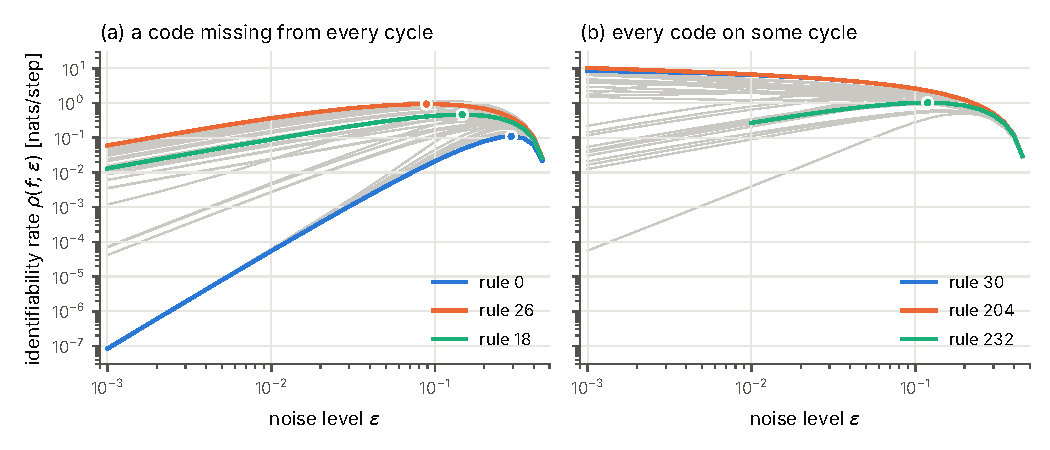
\includegraphics[width=\textwidth]{figures/fig_rates.pdf}
\caption{Identifiability rate $\rho(f;\eps)=\lambda(\eps)\min_c\nu_c(f;\eps)$ for all $88$ classes (grey) with three named rules per panel; dots mark $\eps^*$. (a) Classes in which some code occurs on no cycle: $\rho\to0$ at both ends (Lemma~\ref{lem:ends}). (b) Classes in which every code occurs on some cycle: the curve either still has an interior maximum or keeps rising as $\eps\to0$; the eight coinciding top curves are the affine rules with uniform three-cell marginals, $\rho=\tfrac n8\lambda(\eps)$.}
\label{fig:rates}
\end{figure}

Figure~\ref{fig:rates} shows the exact rate curves. All \NumClassesBproved{} classes with a code absent from every cycle have an interior maximum and fall towards $\eps\to0$ (the ratio of $\rho$ at the two smallest resolved noise levels is at least \FallingBTrendMin), as Lemma~\ref{lem:ends} requires. Among the \NumClassesUndet{} classes whose cycles jointly cover all codes, \NumFallingU{} also fall towards $\eps\to0$ and have an interior maximum---their noise-selected cycles evidently miss a code---while \NumRisingU{} rise as $\eps$ decreases (ratio in $[\RisingTrendMin,\RisingTrendMax]$), consistent with the unbounded branch of Lemma~\ref{lem:ends}. \NumUniformMarginal{} of the rising classes (rules \UniformMarginalRules) have $\nu_c=n/8$ for every code at every grid point (largest deviation \UniformMarginalMaxDev), hence $\rho(f;\eps)=\tfrac n8\lambda(\eps)$ (\UniformMarginalRhoSmall{} at $\eps=0.001$, where $\lambda=\LambdaSmall$); these eight curves coincide. All eight global maps are affine over $\mathrm{GF}(2)$. For \NumBijective{} of them (rules \BijectiveRules) the map is a bijection of $S$ and the uniform law is stationary. For the other \NumAffineNonBij{} (rules \AffineNonBijRules, the additive rules, with kernels of dimension \AffineKernelDims{} on the ring of $12$) the stationary law is not uniform (its smallest entry at $\eps=0.1$ is \AffineMinPi), but its three-cell marginals are: for $F_fx=Lx+b$ the stationary law satisfies $\hat\pi(\chi)=(1-2\eps)^{|\chi|}(-1)^{\chi\cdot b}\hat\pi(L^{\!\top}\chi)$ in the Walsh basis, so $\hat\pi(\chi)=0$ unless some power of $L^{\!\top}$ annihilates $\chi$, and the three-cell marginal at $(i-1,i,i+1)$ is uniform iff $\hat\pi$ vanishes on the nonzero characters supported there; for the four rules the generalised kernel of $L^{\!\top}$ contains \AffineBadCharacters{} such characters (checked by enumeration). On the grid every curve is monotone or unimodal except \NumSignChangesGtOne{} (rules \SignChangesGtOneRules), which rise towards $\eps\to0$, dip, and have a local maximum in between; unimodality is observed, not proved.

For the \NumInterior{} classes that fall towards $\eps\to0$, the interior maxima lie at $\eps^*\in[\EpsStarMin,\EpsStarMax]$ (median \EpsStarMedian; smallest for rule \EpsStarMinRule, largest for rule \EpsStarMaxRule), with peak rates $\rho^*\in[\RhoStarMin,\RhoStarMax]$ nats per step (smallest for rule \RhoStarMinRule, largest for rule \RhoStarMaxRule). Rule $0$, whose only cycle is the all-zero state, is the extreme case: the rarest code is $111$, which requires three adjacent flips, $\nu_7=12\eps^3$, and the maximum sits at $\eps^*=\RuleZeroEpsStar$ with $\rho^*=\RuleZeroRhoStar$ nats per step---at that noise level the observer needs about \RuleZeroStepsPerNat{} steps to accumulate one nat of evidence against the rule that differs from $0$ on $111$. Rules $30$ and $110$ belong to the rising classes: their rates are \RhoSmallRuleThirty{} and \RhoSmallRuleOneTen{} nats per step at $\eps=0.001$ and \RhoMidRuleThirty{} and \RhoMidRuleOneTen{} at $\eps=0.1$; for them noise only lowers the rate. All classes are listed in Appendix~\ref{app:table}. Figure~\ref{fig:zero}(b) relates $\eps^*$ to the zero-noise coverage over these \NumInterior{} falling classes: the classes whose orbits identify the rule from fewer initial states tend to need more noise (Spearman rank correlation \SpearmanEpsStarFrac{} with the identification fraction, $p=\SpearmanPFrac$; \SpearmanEpsStarClass{} with the mean class size, $p=\SpearmanPClass$). At $\eps^*$ the rarest code is $111$ for \ArgminSevenCount{} of the \NumInterior{} classes and $000$ for \ArgminZeroCount: three adjacent equal cells are what noise has to create.

\subsection{Finite horizon}

\begin{figure}[t]
\centering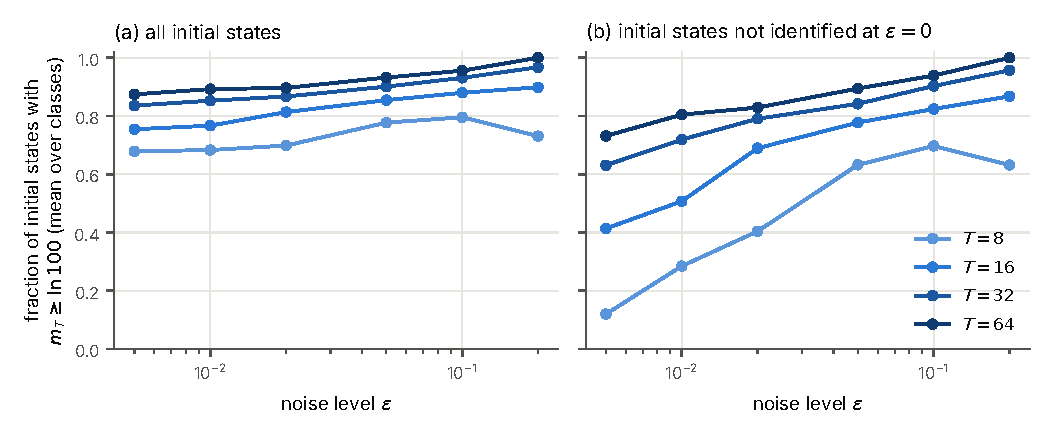
\includegraphics[width=\textwidth]{figures/fig_finite.pdf}
\caption{Fraction of initial states whose evidence margin $m_T(f;x_0,\eps)$ against the hardest alternative reaches $\ln100\approx\FHlnThreshold$ nats within $T$ steps, averaged over the $88$ classes. (a) all initial states; (b) only the initial states that never identify the rule at $\eps=0$. Exact values for $\eps\in\{0.005,0.01,0.02,0.05,0.1,0.2\}$.}
\label{fig:finite}
\end{figure}

The rate is an asymptotic statement; Figure~\ref{fig:finite} shows the exact finite-horizon margins from every initial state. All percentages in this paragraph are means over the $88$ classes of the per-class fraction of initial states. At $\eps=0.005$ and $T=8$, \FHallaA\% of initial states have $m_T\ge\ln100$; at $T=64$ the fraction is \FHallaD\%. Restricted to the initial states that are permanently non-identifiable at $\eps=0$---which have $m_T=0$ for all $T$ without noise, and of which a class has between \FHnonIdStatesPerClassMin{} and \FHnonIdStatesPerClassMax---the fraction rises from \FHgtaA\% ($T=8$) to \FHgtaD\% ($T=64$) at $\eps=0.005$, and at $\eps=0.2$ from \FHgteA\% to \FHgteD\%. Pooled over all such initial states instead of averaged over classes, the $T=32$ fractions are \FHpooledGtaC\% at $\eps=0.005$ and \FHpooledGteC\% at $\eps=0.2$ (class averages \FHgtaC\% and \FHgteC\%). The noise level among the six computed that maximises the worst-case margin over initial states at $T=32$ is, per class, \FHbestEpsHist{} (median $\eps=\FHbestEpsMedian$, against a median $\eps^*=\EpsStarMedian$ for the interior maxima of the rate): at a horizon of a few dozen steps the transient, not the stationary frequency, decides how much noise is useful.

\section{Boundary check: a generator outside the family}\label{sec:boundary}

\begin{figure}[t]
\centering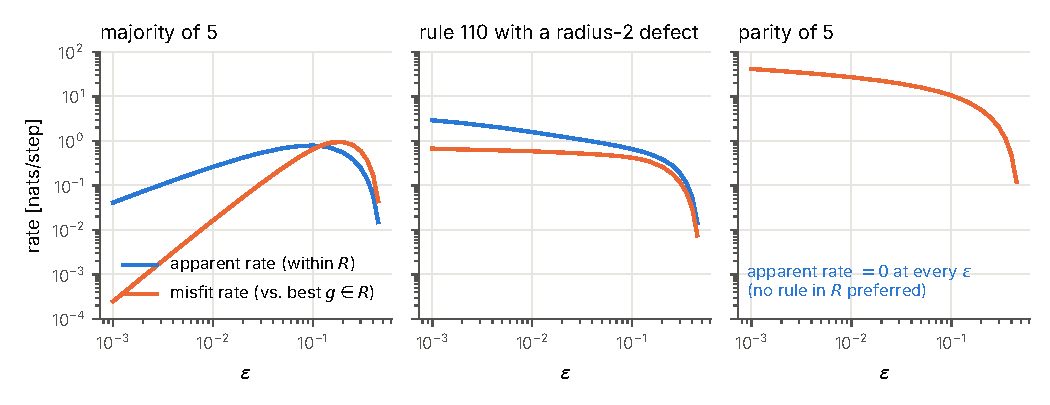
\includegraphics[width=\textwidth]{figures/fig_boundary.pdf}
\caption{Three radius-2 generators scored by the radius-1 observer. Blue: the rate at which the posterior over $\R$ concentrates on the best rule $g^*\in\R$ (apparent identifiability). Orange: the relative-entropy rate between the true chain and the chain of $g^*$ (the evidence that the family is wrong, available to a goodness-of-fit test).}
\label{fig:boundary}
\end{figure}

The definitions assume $f\in\R$. To see what the observer sees when this fails, three radius-2 rules were run through the same chain: the majority of five cells, the parity of five cells, and rule $110$ with its output inverted on the single five-cell context $10101$ (a rule that is radius-1 except on one context). None is reducible to radius 1. Lemma~\ref{lem:decomp} holds for any two deterministic maps under the same noise, so with $a_{c,v}=\E_\pi[\#\{i:\text{code}_i=c,\ (F_hx)_i=v\}]$ the best in-family rule is $g^*(c)=\arg\max_va_{c,v}$, the posterior over $\R$ concentrates on $g^*$ at the rate $\lambda(\eps)\min_c|a_{c,1}-a_{c,0}|$ (``apparent'' rate), and the relative-entropy rate between the true chain and $g^*$'s chain is $\lambda(\eps)\sum_c\min_va_{c,v}$ (``misfit'' rate). At $\eps=0$ the question is whether the orbit is consistent with \emph{some} radius-1 rule.

\begin{table}[h]
\centering\footnotesize\setlength{\tabcolsep}{4pt}
\begin{tabular}{@{}lrrrrrr@{}}\toprule
 & & & \multicolumn{3}{c}{apparent/misfit at $\eps=$} & misfit $>$ apparent\\
generator & silent at $\eps=0$ & $g^*$ & $0.001$ & $0.01$ & $0.2$ & from $\eps=$\\\midrule
majority of 5 & \RiiMajSilent\% & \RiiMajGstarSmall & \RiiMajRatioSmall & \RiiMajRatioMid & \RiiMajRatioLarge & \RiiMajCrossEps\\
rule 110, defect on 10101 & \RiiDefSilent\% & \RiiDefGstarSmall & \RiiDefRatioSmall & \RiiDefRatioMid & \RiiDefRatioLarge & \RiiDefCrossEps\\
parity of 5 & \RiiParSilent\% & tie & \RiiParRatioSmall & \RiiParRatioMid & \RiiParRatioLarge & \RiiParCrossEps\\
\bottomrule
\end{tabular}
\caption{Silent: fraction of the $4096$ initial states whose zero-noise orbit is consistent with some radius-1 rule, so that the misspecification is never detected. $g^*$: the radius-1 rule the posterior concentrates on (the same at every $\eps$ for the first two generators; a tie for parity). Ratios: apparent rate divided by misfit rate.}
\label{tab:boundary}
\end{table}

For the majority rule the observer converges to rule $232$ (majority of three) and, at $\eps=0.01$, accumulates evidence for it \RiiMajRatioMid{} times faster than evidence that the family is wrong; from \RiiMajSilent\% of initial states the zero-noise orbit never reveals the misspecification at all, while from the others it is revealed within the first two transitions. For the defective rule $110$ the observer converges to rule $110$ at every noise level, the misspecification being visible only through the context $10101$. Parity of five is the opposite extreme: the deterministic map is a bijection, the stationary law is uniform, every radius-1 rule mismatches half of the positions, the posterior over $\R$ does not concentrate at all, and the misfit rate is maximal. Within the family, identifiability is a rate that noise can raise; outside it, the same noise raises the apparent rate and the misfit rate together, and which one wins depends on the generator. The observer's posterior alone cannot tell the two situations apart; only a check of the residual flip rate against the declared $\eps$ can.

\section{What is established, and what is not}

Established exactly for $n=12$: the zero-noise classes and closure times for all $256\times4096$ pairs; the rate curves $\rho(f;\eps)$ on the grid for all classes, with the resolved/unresolved status of every entry; $\eps^*$ and $\rho^*$ for every class with an interior maximum; the finite-horizon margins for all initial states at the listed $\eps$ and $T$; the boundary check. Proved for all $n$: Lemmas~\ref{lem:decomp}--\ref{lem:ends}. Observed, not proved: unimodality of the curves; the classification of the \NumClassesUndet{} classes whose cycles jointly cover all codes, which rests on the trend of $\rho$ between the two smallest resolved noise levels (at most \TrendSecondEpsMax; above $0.001$ only for rules \TrendLateRules) and would need the large-deviation weights of the cycles for a proof. Not claimed: anything about $n\ne12$ (the attractor structure of elementary automata changes with the ring size \citep{WuenscheLesser1992}), about observers who do not know $\eps$ or see only part of the ring, or about generators outside the family beyond the three checks of Section~\ref{sec:boundary}.

The practical reading is narrow: for a deterministic system whose attractor exercises only part of its rule, a known amount of dynamical noise is an instrument, not a nuisance, and the right amount can be computed from the rule's stationary neighbourhood frequencies. For a system whose attractor already exercises the whole rule, noise is only a nuisance. Which of the two one is facing can be read off the stationary neighbourhood frequencies; whether the family is the right one cannot be read off the posterior over it.

\subsection*{Statement on the use of AI}
The definitions, the code, the computation, the figures and the text of this note were produced by Claude (Anthropic) in sessions directed by the author on 4 and 15 October 2026. A separate Claude session that had not seen the work recomputed samples of every quantity from the definitions, checked every number in the text against the data files and read the proofs; its findings (among them a false claim that four additive rules are bijections) were corrected in this version, and its report accompanies the code. The author selected the question, set the scope, and is responsible for the content.

\subsection*{Code and data}
The archive accompanying this note contains the code (\texttt{code/}, Python with NumPy), all data files (\texttt{data/}, with \texttt{MANIFEST.sha256}), and a script that regenerates every number and figure in this note from the data files, so that no number here is typed by hand. Repository: \url{https://github.com/frnkptrln/eca-noise-identifiability}; this version is archived as \href{https://doi.org/10.5281/zenodo.23399101}{doi:10.5281/zenodo.23399101}.

\begin{thebibliography}{9}\small
\bibitem[Bretagnolle and Huber(1979)]{BretagnolleHuber1979} J.~Bretagnolle and C.~Huber. Estimation des densit\'es: risque minimax. \emph{Zeitschrift f\"ur Wahrscheinlichkeitstheorie und verwandte Gebiete}, 47:119--137, 1979.
\bibitem[Cover and Thomas(2006)]{CoverThomas} T.~M. Cover and J.~A. Thomas. \emph{Elements of Information Theory}. Wiley, 2nd edition, 2006.
\bibitem[Freidlin and Wentzell(2012)]{FreidlinWentzell} M.~I. Freidlin and A.~D. Wentzell. \emph{Random Perturbations of Dynamical Systems}. Springer, 3rd edition, 2012.
\bibitem[Li and Packard(1990)]{LiPackard1990} W.~Li and N.~Packard. The structure of the elementary cellular automata rule space. \emph{Complex Systems}, 4:281--297, 1990.
\bibitem[Norris(1997)]{Norris} J.~R. Norris. \emph{Markov Chains}. Cambridge University Press, 1997.
\bibitem[Tsybakov(2009)]{Tsybakov2009} A.~B. Tsybakov. \emph{Introduction to Nonparametric Estimation}. Springer, 2009.
\bibitem[Wolfram(1983)]{Wolfram1983} S.~Wolfram. Statistical mechanics of cellular automata. \emph{Reviews of Modern Physics}, 55:601--644, 1983.
\bibitem[Wuensche and Lesser(1992)]{WuenscheLesser1992} A.~Wuensche and M.~Lesser. \emph{The Global Dynamics of Cellular Automata}. Addison-Wesley, 1992.
\end{thebibliography}

\clearpage
\appendix
\section{All 88 classes}\label{app:table}
\footnotesize\setlength{\tabcolsep}{2.6pt}
Columns: class representative $f$ (smallest rule number in the class); type (B: some code occurs on no cycle, so $\rho\to0$ as $\eps\to0$ by Lemma~\ref{lem:ends}; U: every code occurs on some cycle); id.\%: fraction of the $4096$ initial states that determine the rule at $\eps=0$; $\overline{|C_\infty|}$: mean zero-noise class size; $\tau_{\max}$: longest transient plus period; cycles: number of cycles of $F_f$; $|\bigcup N|$: number of codes occurring on cycles; $\eps^*$, $\rho^*$: location and value of the interior maximum of $\rho$ ($\to0$: the largest resolved rate is at the smallest noise level and still rising; $\dagger$: a local maximum, the curve rises again as $\eps\to0$).

\medskip
{\scriptsize% generated by code/make_numbers.py -- do not edit
\begin{tabular}{@{}rcrrrrrrr@{}}\toprule
$f$ & type & id.\,\% & $\overline{|C_\infty|}$ & $\tau_{\max}$ & cycles & $|\bigcup N|$ & $\varepsilon^*$ & $\rho^*$\\\midrule
0 & B & 34.0 & 2.97 & 2 & 1 & 1 & 0.292 & 0.110 \\
1 & B & 63.1 & 1.79 & 3 & 162 & 7 & 0.111 & 0.766 \\
2 & B & 43.4 & 2.69 & 13 & 11 & 4 & 0.234 & 0.200 \\
3 & B & 65.8 & 1.77 & 25 & 39 & 7 & 0.113 & 0.869 \\
4 & B & 38.8 & 2.86 & 2 & 322 & 5 & 0.210 & 0.225 \\
5 & U & 73.1 & 1.79 & 3 & 435 & 8 & $\to 0$ & -- \\
6 & B & 51.4 & 1.80 & 18 & 28 & 7 & 0.146 & 0.485 \\
7 & U & 88.2 & 1.40 & 31 & 10 & 8 & 0.103 & 1.604 \\
8 & B & 50.5 & 2.32 & 3 & 1 & 1 & 0.283 & 0.143 \\
9 & U & 99.0 & 1.08 & 26 & 14 & 8 & $\to 0$ & -- \\
10 & B & 50.5 & 2.54 & 13 & 31 & 6 & 0.167 & 0.358 \\
11 & B & 78.0 & 1.48 & 16 & 32 & 7 & 0.114 & 0.968 \\
12 & B & 50.5 & 2.45 & 2 & 322 & 5 & 0.192 & 0.308 \\
13 & B & 74.1 & 1.58 & 11 & 30 & 6 & 0.111 & 0.937 \\
14 & B & 53.7 & 1.97 & 16 & 36 & 7 & 0.111 & 0.776 \\
15 & U & 84.3 & 1.54 & 12 & 352 & 8 & $\to 0$ & -- \\
18 & B & 56.2 & 1.97 & 38 & 20 & 7 & 0.147 & 0.465 \\
19 & B & 73.7 & 1.72 & 4 & 162 & 6 & 0.120 & 1.039 \\
22 & U & 95.5 & 1.29 & 24 & 23 & 8 & $\to 0$ & -- \\
23 & U & 66.2 & 1.85 & 7 & 164 & 8 & 0.119 & 1.040 \\
24 & B & 58.0 & 2.15 & 14 & 11 & 4 & 0.218 & 0.277 \\
25 & U & 99.8 & 1.06 & 34 & 21 & 8 & $\to 0$ & -- \\
26 & B & 77.0 & 1.50 & 33 & 64 & 7 & 0.088 & 0.941 \\
27 & U & 94.9 & 1.19 & 29 & 44 & 8 & $\to 0$ & -- \\
28 & B & 60.2 & 1.63 & 12 & 75 & 7 & 0.103 & 0.799 \\
29 & U & 85.6 & 1.36 & 3 & 751 & 8 & $\to 0$ & -- \\
30 & U & 99.5 & 1.09 & 228 & 12 & 8 & $\to 0$ & -- \\
32 & B & 50.5 & 2.52 & 7 & 2 & 3 & 0.278 & 0.149 \\
33 & U & 78.7 & 1.40 & 7 & 163 & 8 & 0.116 & 0.916 \\
34 & B & 50.5 & 2.45 & 13 & 31 & 5 & 0.192 & 0.308 \\
35 & U & 63.1 & 1.71 & 29 & 42 & 8 & 0.069 & 1.638 \\
36 & B & 67.9 & 2.01 & 3 & 98 & 4 & 0.149 & 0.443 \\
37 & U & 94.3 & 1.23 & 23 & 58 & 8 & $\to 0$ & -- \\
38 & B & 76.6 & 1.40 & 14 & 52 & 7 & 0.102 & 1.016 \\
40 & B & 50.5 & 2.44 & 12 & 5 & 5 & 0.257 & 0.224 \\
41 & U & 98.8 & 1.20 & 38 & 28 & 8 & 0.035$^\dagger$ & 2.287$^\dagger$ \\
42 & B & 33.7 & 3.02 & 13 & 132 & 7 & 0.132 & 0.626 \\
43 & U & 48.3 & 2.11 & 15 & 61 & 8 & 0.056 & 2.062 \\
44 & B & 79.1 & 1.74 & 7 & 99 & 7 & 0.124 & 0.760 \\
45 & U & 99.7 & 1.09 & 240 & 33 & 8 & $\to 0$ & -- \\
46 & B & 64.9 & 1.76 & 14 & 11 & 6 & 0.107 & 1.123 \\
50 & B & 63.4 & 1.79 & 8 & 163 & 7 & 0.102 & 0.804 \\
51 & U & 84.3 & 1.54 & 2 & 2048 & 8 & $\to 0$ & -- \\
54 & U & 98.0 & 1.10 & 25 & 33 & 8 & $\to 0$ & -- \\
\bottomrule\end{tabular}\hspace{1.2em}
\begin{tabular}{@{}rcrrrrrrr@{}}\toprule
$f$ & type & id.\,\% & $\overline{|C_\infty|}$ & $\tau_{\max}$ & cycles & $|\bigcup N|$ & $\varepsilon^*$ & $\rho^*$\\\midrule
56 & B & 47.8 & 2.55 & 17 & 34 & 7 & 0.138 & 0.582 \\
57 & U & 71.6 & 1.68 & 20 & 8 & 8 & 0.105 & 1.263 \\
58 & U & 62.4 & 1.83 & 27 & 9 & 8 & 0.109 & 1.178 \\
60 & U & 99.8 & 1.08 & 16 & 24 & 8 & $\to 0$ & -- \\
62 & U & 96.9 & 1.16 & 29 & 92 & 8 & $\to 0$ & -- \\
72 & B & 56.1 & 2.37 & 3 & 98 & 6 & 0.233 & 0.250 \\
73 & U & 89.8 & 1.22 & 14 & 162 & 8 & $\to 0$ & -- \\
74 & U & 91.9 & 1.83 & 21 & 29 & 8 & $\to 0$ & -- \\
76 & B & 38.7 & 2.94 & 2 & 1499 & 7 & 0.135 & 0.596 \\
77 & U & 56.1 & 2.07 & 6 & 325 & 8 & 0.119 & 1.040 \\
78 & B & 74.1 & 1.60 & 12 & 30 & 5 & 0.120 & 1.145 \\
90 & U & 93.2 & 1.40 & 6 & 70 & 8 & $\to 0$ & -- \\
94 & U & 82.7 & 1.53 & 12 & 147 & 8 & 0.070 & 1.511 \\
104 & U & 76.8 & 2.15 & 10 & 50 & 8 & 0.195 & 0.508 \\
105 & U & 98.9 & 1.13 & 6 & 10 & 8 & $\to 0$ & -- \\
106 & U & 91.7 & 1.90 & 168 & 37 & 8 & 0.010 & 6.189 \\
108 & U & 75.6 & 1.84 & 4 & 674 & 8 & $\to 0$ & -- \\
110 & U & 99.0 & 1.09 & 44 & 11 & 8 & $\to 0$ & -- \\
122 & U & 75.7 & 1.59 & 41 & 21 & 8 & $\to 0$ & -- \\
126 & B & 76.4 & 1.40 & 38 & 20 & 7 & 0.108 & 0.862 \\
128 & B & 47.6 & 2.53 & 7 & 2 & 2 & 0.293 & 0.130 \\
130 & B & 63.4 & 2.27 & 17 & 12 & 5 & 0.236 & 0.244 \\
132 & B & 46.8 & 2.58 & 6 & 323 & 6 & 0.217 & 0.264 \\
134 & U & 63.4 & 1.55 & 19 & 29 & 8 & 0.148 & 0.609 \\
136 & B & 50.5 & 2.34 & 12 & 2 & 2 & 0.270 & 0.201 \\
138 & B & 37.4 & 2.82 & 13 & 77 & 7 & 0.123 & 0.821 \\
140 & B & 50.5 & 2.47 & 11 & 323 & 6 & 0.188 & 0.450 \\
142 & U & 23.1 & 2.39 & 15 & 61 & 8 & 0.056 & 2.062 \\
146 & U & 63.2 & 1.68 & 39 & 21 & 8 & 0.157 & 0.567 \\
150 & U & 97.9 & 1.15 & 6 & 10 & 8 & $\to 0$ & -- \\
152 & B & 63.4 & 2.11 & 23 & 12 & 5 & 0.204 & 0.429 \\
154 & U & 64.5 & 1.72 & 24 & 308 & 8 & $\to 0$ & -- \\
156 & U & 34.7 & 1.90 & 11 & 76 & 8 & 0.107 & 1.253 \\
160 & B & 47.5 & 2.66 & 7 & 3 & 4 & 0.276 & 0.188 \\
162 & B & 43.9 & 2.72 & 17 & 32 & 6 & 0.185 & 0.430 \\
164 & U & 64.9 & 2.16 & 6 & 108 & 8 & 0.152 & 0.625 \\
168 & B & 43.4 & 3.14 & 12 & 32 & 6 & 0.232 & 0.386 \\
170 & U & 19.0 & 3.93 & 12 & 352 & 8 & $\to 0$ & -- \\
172 & U & 71.3 & 2.48 & 13 & 109 & 8 & 0.122 & 1.163 \\
178 & U & 34.7 & 2.28 & 7 & 164 & 8 & 0.119 & 1.040 \\
184 & U & 34.7 & 3.31 & 16 & 61 & 8 & $\to 0$ & -- \\
200 & B & 38.8 & 3.14 & 2 & 853 & 7 & 0.173 & 0.591 \\
204 & U & 19.0 & 3.93 & 1 & 4096 & 8 & $\to 0$ & -- \\
232 & U & 50.7 & 3.33 & 6 & 325 & 8 & 0.119 & 1.040 \\
\bottomrule\end{tabular}
}

\end{document}
